%!TEX root = ../thesis.tex
%*******************************************************************************
%****************************** Third Chapter **********************************
%*******************************************************************************
\chapter{Precise Shape Reconstructions}

% **************************** Define Graphics Path **************************
\ifpdf
    \graphicspath{{Chapter4/Figs/Raster/}{Chapter4/Figs/PDF/}{Chapter4/Figs/}}
\else
    \graphicspath{{Chapter4/Figs/Vector/}{Chapter4/Figs/}}
\fi

\section{First section of the third chapter}
And now I begin my third chapter here \dots

And now to cite some more people~\citet{Rea85,Ancey1996}


\section{Abstract}
  We introduce an automatic, end-to-end method for recovering the 3D pose and shape of dogs from monocular internet images. 
  The large variation in shape between dog breeds, significant occlusion and low quality of internet images makes this a challenging problem.
  We learn a richer prior over shapes than previous work, which helps regularize parameter estimation.
  We demonstrate results on the Stanford Dog Dataset, an `in the wild' dataset of 20,580 dog images for which we have collected 2D joint and silhouette annotations to split for training and evaluation. 
  In order to capture the large shape variety of dogs, we show that the natural variation in the 2D dataset is enough to learn a detailed 3D prior through expectation maximization (EM).
  As a by-product of training, we generate a new parameterized model (including limb scaling) SMBLD which we release alongside our new annotation dataset \emph{StanfordExtra} to the research community.
    
\section{Introduction}
  Animals contribute greatly to our society, in numerous ways both economic and otherwise (there are more than 63 million pet dogs in the US alone~\cite{appa20}).
  Consequently, there has been considerable attention in the computer vision research community to the interpretation of animal imagery.
  Although these techniques share similarities to those used for understanding images of humans, a key difference is that obtaining labelled training data for animals is more difficult than for humans. This is due to the wide range of shapes and species of animals, and the difficulty of educating manual labellers in animal physiology.
  \begin{figure}[t]
  \setlength{\fboxsep}{0pt}%
\setlength{\fboxrule}{0pt}%

% Define left and right aligned fixed width columns
\renewcommand\tabularxcolumn[1]{m{#1}}% for vertical centering text in X column
\newcolumntype{L}[1]{>{\hsize=#1\hsize\raggedright\arraybackslash}X}%
\renewcommand\tabularxcolumn[1]{m{#1}}% for vertical centering text in X column
\newcolumntype{R}[1]{>{\hsize=#1\hsize\raggedleft\arraybackslash}X}%

\begin{tabularx}{1\textwidth}{@{} *{3}{R{0.1666}L{0.1666}}@{}p{0cm} @{}}

    \includegraphics[height=0.2\linewidth, max width=0.15\linewidth]{ours_sup/n02088632-bluetick/orig/n02088632_744_crop.jpg} &
    \includegraphics[height=0.2\linewidth, max width=0.15\linewidth]{ours_sup/n02088632-bluetick/fit/n02088632_744_crop.jpg} &

    \includegraphics[height=0.2\linewidth, max width=0.15\linewidth, max width=0.15\linewidth]{ours_sup/n02087394-Rhodesian_ridgeback/orig/n02087394_5552_crop.jpg} &
    \includegraphics[height=0.2\linewidth, max width=0.15\linewidth, max width=0.15\linewidth]{ours_sup/n02087394-Rhodesian_ridgeback/fit/n02087394_5552_crop.jpg} &

    \includegraphics[height=0.2\linewidth, max width=0.15\linewidth]{ours_sup/n02108422-bull_mastiff/orig/n02108422_4039_crop.jpg} &
    \includegraphics[height=0.2\linewidth, max width=0.15\linewidth]{ours_sup/n02108422-bull_mastiff/fit/n02108422_4039_crop.jpg} &



    \\

    \includegraphics[height=0.2\linewidth, max width=0.15\linewidth]{ours_sup/n02099429-curly-coated_retriever/orig/n02099429_2570_crop.jpg} &
    \includegraphics[height=0.2\linewidth, max width=0.15\linewidth]{ours_sup/n02099429-curly-coated_retriever/fit/n02099429_2570_crop.jpg} &

    \includegraphics[height=0.2\linewidth, max width=0.15\linewidth]{ours_sup/n02091244-Ibizan_hound/orig/n02091244_3373_crop.jpg} &
    \includegraphics[height=0.2\linewidth, max width=0.15\linewidth]{ours_sup/n02091244-Ibizan_hound/fit/n02091244_3373_crop.jpg} &

    \includegraphics[height=0.2\linewidth, max width=0.15\linewidth]{ours_sup/n02087046-toy_terrier/orig/n02087046_133_crop.jpg} &
    \includegraphics[height=0.2\linewidth, max width=0.15\linewidth]{ours_sup/n02087046-toy_terrier/fit/n02087046_133_crop.jpg} &

    \\
    \includegraphics[height=0.2\linewidth, max width=0.15\linewidth]{ours_sup/n02097658-silky_terrier/orig/n02097658_6672.jpg} &
    \includegraphics[height=0.2\linewidth, max width=0.15\linewidth]{ours_sup/n02097658-silky_terrier/fit/n02097658_6672.jpg} &

    \includegraphics[height=0.2\linewidth, max width=0.15\linewidth]{ours_sup/n02110806-basenji/orig/n02110806_2957_crop.jpg} &
    \includegraphics[height=0.2\linewidth, max width=0.15\linewidth]{ours_sup/n02110806-basenji/fit/n02110806_2957_crop.jpg} &

    \includegraphics[height=0.2\linewidth, max width=0.15\linewidth]{ours_sup/n02089973-English_foxhound/orig/n02089973_1763_crop.jpg} &
    \includegraphics[height=0.2\linewidth, max width=0.15\linewidth]{ours_sup/n02089973-English_foxhound/fit/n02089973_1763_crop.jpg}  &  

\end{tabularx}\medbreak
  \caption{
  \textbf{End-to-end 3D dog reconstruction from monocular images.}
  We propose a novel method that, given a monocular input image of a dog, directly predicts a set of SMBLD parameters to generate an accurate 3D dog model consistent in terms of shape and pose with the input. 
  We regularize learning using a multi-modal shape prior, which is tuned during training with an expectation maximization scheme.\label{fig:splash}}
  \end{figure}
  
  Dogs are a particular species of interest, however it is noticeable that existing work has not yet demonstrated effective 3D reconstruction of dogs over large test sets.
  We postulate that this is partially because dog breeds are remarkably dissimilar in shape and texture, presenting a challenge to the current state of the art.
  The methods we propose extend the state of the art in several ways.
  While each of these qualities exist in some existing works, we believe ours is the first to exhibit this combination, leading to a new state of the art in terms of scale and object diversity.
  \begin{enumerate}
      \item We reconstruct pose and shape on a test set of 1703 low-quality internet images of a complex 3D object class (dogs).
      \item We directly regress to object pose and shape from a single image without a model fitting stage.
      \item We use easily obtained 2D annotations in training, and none at test time.
      \item We incorporate fitting of a new multi-modal prior into the training phase (via EM update steps), rather than fitting it to 3D data as in previous work.
      \item We introduce new degrees of freedom to the SMAL model, 
      allowing explicit scaling of subparts.
  \end{enumerate}
  
  \subsection{Related work}
  
  The closest work in terms of scale is the category-specific mesh reconstruction of Kanazawa et al.~\cite{kanazawa2018birds}, where 2850 images of birds were reconstructed.  However, doing so for the complex pose and shape variations of dogs required the advances described in this paper.
  
  Table~\ref{tab:literature} summarizes previous work on animal reconstruction.
  It is interesting to note that while several papers demonstrate reconstruction across species, which {\em prima facie} is a richer class than just dogs, the test-time requirements (e.g. manually-clicked keypoints/silhouette segmentations, input image quality etc.) are considerably higher for those systems.
  Thus we claim that the achievement of reconstructing a full range of dog breeds, 
  with variable fur length, varying shape and pose of ears, and with considerable occlusion, is a significant contribution.
  
  \newcolumntype{L}[1]{>{\RaggedRight\hspace{0pt}}p{#1}}
  \newcolumntype{R}[1]{>{\RaggedLeft\hspace{0pt}}p{#1}}
  
  \newcommand{\awfhang}[1]{
  \begin{minipage}[t]{\textwidth}% Top-hanging minipage, will align on
                                 % bottom of first line
  \begin{tabbing} % tabbing so that minipage shrinks to fit
  \\[-\baselineskip] % Make first line zero-height
  #1 % Include user's text
  \end{tabbing}
  \end{minipage}} % can't allow } onto next line, as {WIDEBOX}~x will not tie.
  
  
  \begin{table}[t!]
  {\sffamily
  \scriptsize
  \def\hd#1{\awfhang{#1}}
  \begin{tabular}{@{}L{20mm}%Paper
  |L{12mm}%Class
  L{15mm}%Train
  |L{15mm}%Template
  L{17mm}%Video
  L{17mm}%Test
  |L{9mm}%Model
  L{6mm}%Size
  @{}}
  \hd{Paper}%
  &\hd{Animal\\Class}%
  &\hd{Training\\requirements}%
  &\hd{Template\\Model}%
  &\hd{Video\\required}%
  &\hd{Test Time\\Annotation}%
  &\hd{Model\\Fitting}%
  &\hd{Test\\Size}%
  \\\hline
  %%%%%%%%%%%%%%%%%%%%%%
  This paper
  & Dogs  % 2D Joints, Silhouettes, 3D Template, 3D Priors
  & J2, S2, T3, P3
  & SMAL
  & No & None & No & 1703
  \\\hline
  %%%%%%%%%%%%%%%%%%%%%%
  3D-Safari~\cite{Zuffi19Safari}        
  & Zebras, horses
  % 3D models (albeit synthetic), 2D Joints,  Silhouettes,  3D Priors
  & M3 (albeit synthetic), J2, S2, P3
  & SMAL
  & 3-7 frames / animal & None & Yes & 200
  \\\hline
  %%%%%%%%%%%%%%%%%%%%%%
  Lions, Tigers and Bears (SMALR)~\cite{Zuffi:CVPR:2018} 
  & MLQ
  & Not trained
  & SMAL
  & 3-7 frames / animal & J2, S2 & Yes & 14
  \\\hline
  %%%%%%%%%%%%%%%%%%%%%%
  3D Menagerie (SMAL)~\cite{DBLP:journals/corr/ZuffiKJB16}                
  & MLQ 
  & Not trained
  & SMAL
  & No & J2, S2 & Yes & 48 
  \\\hline
  %%%%%%%%%%%%%%%%%%%%%%
  Creatures Great and SMAL~\cite{biggs2018creatures}
  & MLQ
  & Not trained
  & SMAL
  & Yes & S2 (for best results shown) & Yes & 9             \\\hline 
  %%%%%%%%%%%%%%%%%%%%%%
  Category Specific Mesh Reconstructions~\cite{kanazawa2018birds}
  & Birds
  & J2, S2
  & Bird convex hull
  & No & None & No & 2850          
  \\\hline
  %%%%%%%%%%%%%%%%%%%%%%
  What Shape are Dolphins~\cite{cashman2013shape}
  & Dolphins, Pigeons 
  & Not trained
  & Dolphin Template
  & 25 frames / category & J2, S2 & Yes & 25
  \\\hline
  %%%%%%%%%%%%%%%%%%%%%%
  Animated 3D Creatures~\cite{reinert2016animatedsketching}
  & MLQ
  & Not trained
  & Generalized Cylinders
  & Yes & J2, S2 & Yes & 15
  \\\hline
  \end{tabular}
  }
  \vspace{1em}
  \caption{Literature summary: Our paper extends large-scale `in the wild' reconstruction to the difficult class of diverse breeds of dogs. 
  MLQ: Medium-to-large quadrupeds. J2: 2D Joints. S2: 2D Silhouettes. T3: 3D Template. P3: 3D Priors. M3: 3D Model.}
  \label{tab:literature}
  \end{table}
  
  \subsubsection{Monocular 3D reconstruction of human bodies}
  The majority of recent work in 3D pose and shape recovery from monocular images tackles the special case of 3D \emph{human} reconstruction. As a result, the research community has collected a multitude of open source human datasets which provide strong supervisory signals for training deep neural networks. These include accurate 3D deformable template models~\cite{loper2015smpl} generated from real human scans, 3D motion capture datasets~\cite{ionescu2013human3,vonMarcard2018} and large 2D datasets~\cite{mscoco,Johnson10,andriluka14cvpr} which provide keypoint and silhouette annotations. 
  
  The abundance of available human data has supported the development of successful monocular 3D reconstruction pipelines~\cite{kolotouros19convolutional,hmrKanazawa17}. Such approaches rely on accurate 3D data to build detailed priors over the distribution of human shapes and poses, and use large 2D keypoint datasets to promote generalization to `in the wild' scenarios. Silhouette data has also been shown to assist in accurate reconstruction of clothes, hair and other appearance detail~\cite{pifuSHNMKL19,alldieck2019learning}.
  While the dominant paradigm in human reconstruction is now end-to-end deep learning methods, SPIN~\cite{kolotouros2019learning} shows impressive improvement by incorporating an energy minimization process within their training loop to further minimize a 2D reprojection loss subject to fixed pose \& shape priors. Inspired by this innovation, we learn an iteratively-improving shape prior by applying expectation maximization during the training process.
  
  \textbf{Monocular 3D reconstruction of animal categories.}
  While animals are often featured in computer vision literature, there are still relatively few works that focus on accurate 3D animal reconstruction. 
  
  A primary reason for this is absence of large scale 3D datasets\footnote{Released after the submission of this paper, RGBD-Dog dataset~\cite{Kearney_2020_CVPR} is the first open-source 3D motion capture dataset for dogs.} stemming from the practical challenges associated with 3D motion capture, as well as a lack of 2D data which captures a wide variety of animals. The recent Animal Pose dataset~\cite{animalpose} is one such 2D alternative, but contains significantly fewer labelled images than in our new StanfordDogs dataset (4,000 compared to 20,580). On the other hand, animal silhouette data is plentiful~\cite{mscoco,everingham2010pascal,DAVIS2017-2nd}.
  
  Zuffi et al.~\cite{DBLP:journals/corr/ZuffiKJB16} made a significant contribution to 3D animal reconstruction research by releasing SMAL, a deformable 3D quadruped model (analagous to SMPL~\cite{loper2015smpl} for human reconstruction) from $41$ scans of artist-designed toy figurines. The authors also released shape and pose priors generated from artist data. In this work we develop \emph{SMBLD}, an extension of SMAL that better represents the diverse dog category by adding scale parameters and refining the shape prior using our large image dataset.
  
  While there have been various `model-free' approaches which do not rely on an initial template model to generate the 3D animal reconstruction, these techniques often do not produce a mesh~\cite{Agudo_2018_CVPR,novotny19c3dpo} or rely heavily on input 2D keypoints or video at test-time~\cite{vicente_3dv,Probst2018_ECCVa}. An exception is the end-to-end network of Kanazawa et al.~\cite{kanazawa2018birds}, although we argue that the bird category exhibits more limited articulation than our dog category.
  
  We instead focus on model-based approaches. The SMAL authors~\cite{DBLP:journals/corr/ZuffiKJB16} demonstrate fitting their deformable 3D model to quadruped species using user-provided keypoint and silhouette dataset. SMALR~\cite{Zuffi:CVPR:2018} then demonstrated fitting to broader animal categories by incorporating multi-view constraints from video sequences. Biggs et al.~\cite{biggs2018creatures} overcame the need for hand-clicked keypoints by training a joint predictor on synthetic data. 3D-Safari~\cite{Zuffi19Safari} further improve by training a deep network on synthetic data (built using SMALR~\cite{Zuffi:CVPR:2018}) to recover detailed zebra shapes `in the wild'.
  
  A drawback of these approaches is their reliance on a test-time energy-based optimization procedure, which is susceptible to failure with poor quality keypoint/silhouette predictions and increases the computational burden. By contrast our method requires no additional energy-based refinement, and is trained purely from single `in the wild' images. The experimental section of this paper contains a robust comparison between our end-to-end method and relevant optimization-based approaches. 
  
  A major impediment to research in 3D animal reconstruction has been the lack of a strong evaluation benchmark, with most of the above methods showing only qualitative evaluations or providing quantitative results on fewer than 50 examples. To remedy this, we introduce \emph{StanfordExtra}, a new large-scale dataset which we hope will drive further progress in the field. 
  
  \input{fig_system_overview_cr}
  
  \section{Parametric animal model}
  
  \def\R#1{{\mathbb{R}^{#1}}}
  \def\RR#1#2{{\mathbb{R}^{#1 \times #2}}}
  \def\posn{\phi}
  \def\pose{\theta}
  \def\npose{P}
  \def\shape{\beta}
  \def\scale{\kappa}
  \def\trans{t}
  \def\betacov{{\Sigma_{\beta}}}
  \def\posecov{{\Sigma_{\pose}}}
  \def\posemean{{\mu_{\pose}}}
  \def\betamean{{\mu_{\beta}}}
  \def\nimages{N}
  \def\nshape{B}
  \def\verts{\nu}
  \def\nverts{V}
  \def\jointselect{\mathtt{K}}
  \def\njoints{J}
  \def\f{f}
  
  At the heart of our method is a parametric representation of a 3D animal mesh, which is based on the Skinned Multi-Animal Linear (SMAL) model proposed by~\cite{DBLP:journals/corr/ZuffiKJB16}. SMAL is a deformable 3D animal mesh parameterized by shape and pose. The \emph{shape}~$\shape \in \R\nshape$ parameters are PCA coefficients of an undeformed template mesh with limbs in default position. The \emph{pose}~$\pose \in \R\npose$ parameters meanwhile govern the joint angle rotations ($35 \times 3$ Rodrigues parameters) which effect the articulated limb movement. The model consists of a linear blend skinning function $F_{v}: (\pose, \shape) \mapsto V$, which generates a set of vertex positions $V \in \RR{3889}{3}$, and a joint function $F_{J}: (\pose, \shape) \mapsto J$, which generates a set of joint positions $J \in \RR{35}{3}$.
  
  \subsection{Introducing scale parameters}
  While SMAL has been shown to be adequate for representing a variety of quadruped types, we find that the modes of dog variation are poorly captured by the current model. This is unsurprising, since SMAL used only four canines in its construction.
  
  We therefore introduce a simple but effective way to improve the model's representational power over this particularly diverse  animal category. We augment the set of shape parameters $\beta$ with an additional set $\scale$ which independently scale parts of the mesh. For each model joint, we define parameters ${\scale_x,\scale_y,\scale_z}$ which apply a local scaling of the mesh along the local coordinate $x, y, z$ axes, before pose is applied. Allowing each joint to scale entirely independently can however lead to unrealistic deformations, so we share scale parameters between multiple joints, e.g. leg lengths. The new Skinned Multi-Breed Linear Model for Dogs (SMBLD) is therefore adapted from SMAL by adding $6$ scale parameters to the existing set of shape parameters. Figure~\ref{fig:shape_variation} shows how introducing scale parameters increases the flexibility of the SMAL model. We also extend the provided SMAL shape prior (which later initializes our EM procedure) to cover the new scale parameters by fitting SMBLD to a set of $13$ artist-designed 3D dog meshes. Further details left to the supplementary.
  
  \begin{figure*}[t!]
    \centering
    % \includegraphics[width=0.23\linewidth]{OllieFigs/mean.png}
    % \includegraphics[width=0.23\linewidth]{OllieFigs/leg_lengthen.png}
    % \includegraphics[width=0.23\linewidth]{OllieFigs/tail_shorten.png}
    % \includegraphics[width=0.23\linewidth]{OllieFigs/tail_puff.png}
    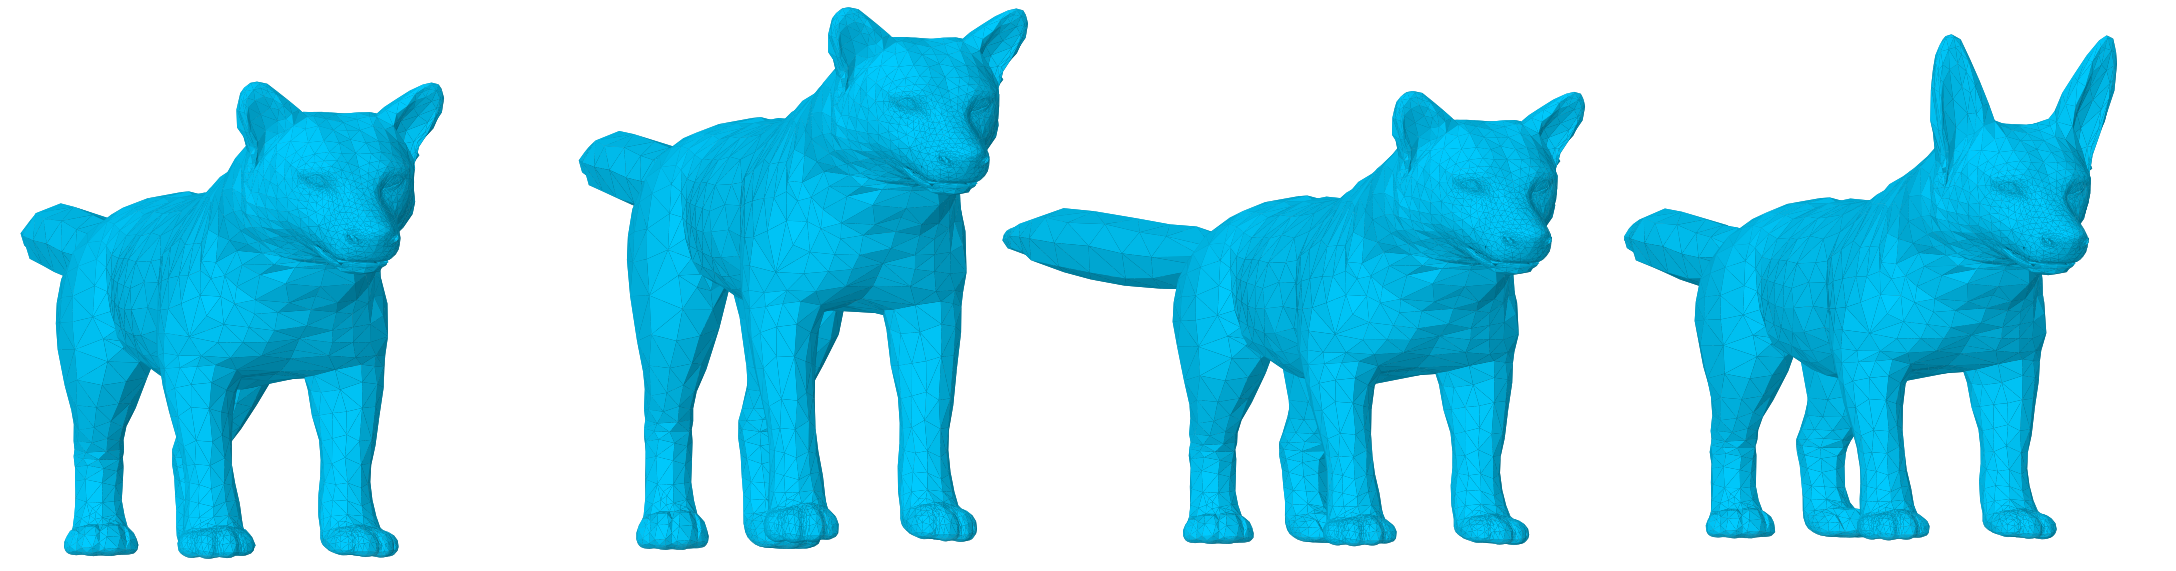
\includegraphics[width=.95\linewidth]{OllieFigs/all_shapevar.png}
    \caption{\textbf{Effect of varying SMBLD scale parameters}. 
    \emph{From left to right}: 
    Mean SMBLD model, 
    25\% leg elongation,
    50\% tail elongation,
    50\% ear elongation.}
    \label{fig:shape_variation}
\end{figure*}
  
  \section{End-to-end dog reconstruction from monocular images} 
  
  We now consider the task of reconstructing a 3D dog mesh from a monocular image. We achieve this by training an end-to-end convolutional network that predicts a set of SMBLD model and perspective camera parameters. In particular, we train our network to predict pose $\pose$ and shape $\shape$ SMBLD parameters together with translation $\trans$ and focal length $f$ for a perspective camera. A complete overview of the proposed system is shown in Figure~\ref{fig:sys_overview_train_sup}.
  
  \subsection{Model architecture}
  
  Our network architecture is inspired by the model of 3D-Safari~\cite{Zuffi19Safari}. Given an input image cropped to (224, 224), we apply a Resnet-50~\cite{he2016deep} backbone network to encode a 1024-dimensional feature map. These features are passed through various linear prediction heads to produce the required parameters. The pose, translation and camera prediction modules follow the design of 3D-Safari, but we describe the differences in our shape module.
  
  \ss{Pose, translation and camera prediction.}
  These modules are independent multi-layer perceptrons which map the above features to the various parameter types. As with 3D-Safari we use two linear layers to map to a set of $35 \times 3$ 3D pose parameters (three parameters for each joint in the SMBLD kinematic tree) given in Rodrigues form. We use independent heads to predict camera frame translation $\trans_{x,y}$ and depth $\trans_{z}$ independently. We also predict the focal length of the perspective camera similarly to 3D-Safari.
  
  \ss{Shape and scale prediction.}
  
  Unlike 3D-Safari, we design our network to predict the set of shape parameters (including scale) rather than vertex offsets. We observe improvement by handling the standard 20 blend-shape parameters and our new scale parameters in separate linear prediction heads. We retrieve the scale parameters by $\scale = \exp{x}$ where $x$ are the network predictions, as we find predicting log scale helps stabilise early training.
  
  \subsection{Training losses}
  
  A common approach for training such an end-to-end system would be to supervise the prediction of $(\pose, \shape, \trans, \f)$ with 3D ground truth annotations~\cite{kolotouros2019learning,kanazawa18end-to-end,pavlakos18learning}. However, building a suitable 3D annotation dataset would require an experienced graphics artist to design an accurate ground truth mesh for each of 20,520 StanfordExtra dog images, a prohibitive expense.
  
  
  We instead develop a method that instead relies on \emph{weak 2D supervision} to guide network training. In particular, we rely on only 2D keypoints and silhouette segmentations, which are significantly cheaper to obtain.
  
  The rest of this section describes the set of losses used to supervise the network at train time.
  
  \ss{Joint reprojection.}
  The most important loss to promote accurate limb positioning is the joint reprojection loss $\L{joints}$, which compares the projected model joints $\pi(F_{J}(\pose, \shape), \trans, \f)$ to the ground truth annotations $\hat{X}$. Given the parameters predicted by the network, we apply the SMBLD model to transform the pose and shape parameters into a set of 3D joint positions $J \in \RR{35}{3}$, and project them to the image plane using translation and camera parameters. The joint loss $L_{joints}$ is given by the $\ell_2$ error between the ground truth and projected joints:
  
  \begin{equation}
  \L{joints}(\pose, \shape, \trans, \f; \hat{X}) = \lVert \hat{X} - \pi(F_{J}(\pose, \shape), \trans, \f) \rVert_{2}
  \end{equation}
  Note that many of our training images exhibit significant occlusion, so $\hat{X}$ contains many invisible joints. We handle this by masking $\L{joints}$ to prevent invisible joints contributing to the loss.
  
  \ss{Silhouette loss.}
  The silhouette loss $\L{sil}$ is used to promote shape alignment between the SMBLD dog mesh and the input dog. In order to compute the silhouette loss, we define a rendering function $R: (\verts, \trans, \f) \mapsto S$ which projects the SMBLD mesh to produce a binary segmentation mask. In order to allow derivatives to be propagated through $R$, we implement $R$ using the differentiable Neural Mesh Renderer~\cite{kato2018renderer}. The loss is computed as the $\ell_2$ difference between a projected silhouette and the ground truth mask $\hat{S}$:
  
  \begin{equation}
  \L{sil}(\pose, \shape, \trans, \f; \hat{S}) = \lVert \hat{S} - R\bigl(F_{V}(\pose, \shape), \trans, \f \bigr) \rVert_{2}
  \end{equation}
  
  
  \ss{Priors.}
  In the absence of 3D ground truth training data, we rely on priors obtained from artist graphics models to encourage realism in the network predictions. We model both pose and shape using a multivariate Gaussian prior, consisting of means $\mu_{\pose},\mu_{\shape}$ and covariance matrices $\Sigma_{\pose},\Sigma_{\shape}$. The loss is given as the log likelihood of a given shape or pose vector under these distributions, which corresponds to the Mahalanobis distance between the predicted parameters and their corresponding means:
  \begin{align}
      \L{pose}(\pose; \mu_{\pose}, \Sigma_{\pose}) &= (\pose - \mu_{\pose})^T \Sigma_{\pose}^{-1} (\pose - \mu_{\pose})\\
      \L{shape}(\shape; \mu_{\shape}, \Sigma_{\shape}) &= (\shape - \mu_{\shape})^T \Sigma_{\shape}^{-1} (\shape - \mu_{\shape})
  \end{align}
  Unlike previous work, we find there is no need to use a loss to penalize pose parameters if they exceed manually specified joint angle limits. We suspect our network learns this regularization naturally because of our large dataset.
  
  
  \subsection{Learning a multi-modal shape prior.}
  
  The previous section introduced a unimodal, multivariate Gaussian shape prior, based on mean $\mu_{\shape}$ and covariance matrix $\Sigma_{\shape}$. However, we find enforcing this prior throughout training tends to result in predictions which appear similar in 3D shape, even when tested on dog images of different breeds. We propose to improve diversity among predicted 3D dog shapes by extending the above formulation to a mixture of $M$ Gaussians prior.  
  The mixture shape loss is then given as:
  \begin{align}
      \L{mixture}(\shape_{i}; \mu_{\shape}, \Sigma_{\shape}, \Pi_{\shape})
      =&
      \sum_{m=1}^M
      \Pi_{\shape}^m
      (\shape_{i} - \mu_{\shape}^{m})^{T} \inv{\Sigma_{\shape}^{m}} (\shape_{i} - \mu_{\shape}^{m})
      \\
      =&
      \sum_{m=1}^M \Pi_{\shape}^{m}\L{shape}(\shape_{i}; \mu_{\shape}^{m}, \Sigma_{\shape}^{m})
  \end{align}
  Where $\mu_{\shape}^{m}$, $\Sigma_{\shape}^{m}$ and $\Pi_{\shape}^{m}$ 
  are the mean, covariance and mixture weight respectively for Gaussian component 
  $m$. For each component the mean is sampled from our existing unimodal prior, and the covariance is set equal to the unimodal prior i.e. $\Sigma_{\shape}^{m} := \Sigma_{\shape}$. All mixture weights are initially set to $\frac{1}{M}$.
  
  Each training image $i$ is assigned a set of latent variables $\{w_{i}^{1}, \dots w_{i}^{M}\}$ encoding the probability of the dog shape in image~$i$ being generated by component~$m$. 
  
  \subsection{Expectation Maximization in the loop}
  
  As previously discussed, our initial shape prior is obtained from artist data which we find is unrepresentative of the diverse shapes present in our real dog dataset. We address this by proposing to recover the latent variables $w_{i}^{m}$ and parameters ($\mu_{\shape}^{m}$, $\Sigma_{\shape}^{m}$ and $\Pi_{\shape}^{m}$) of our 3D shape prior by learning from monocular images of `in the wild' dogs and their 2D training labels in our training dataset.
  
  We achieve this using Expectation Maximization (EM), which regularly updates the means and variances for each mixture component and per-image mixture weights based on the observed shapes in the training set. While training our 3D reconstruction network, we progressively update our shape mixture model with an alternating `E' step and `M' step described below:
  
  \subsubsection{The `E' Step.}
  The `E' step computes the expected value of the latent variables~$w_{i}^{m}$ 
  assuming fixed $(\mu_{\shape}^{m}, \Sigma_{\shape}^{m}, \Pi_{\shape}^{m})$ for all $i \in \{1,\dots,N\}, m \in \{1,\dots,M\}$.
  
  The update equation for an image $i$ with latest shape prediction $\shape_{i}$ 
  and cluster $m$ with parameters $(\mu_{\shape}^{m}, \Sigma_{\shape}^{m}, \Pi_{\shape}^{m})$ 
  is given as:
  
  \begin{align}
      w_{i}^{m} 
      :=& 
      \frac{
          \mathcal{N}(\shape_{i} | \mu_{\shape}^{m},\Sigma_{\shape}^{m})\Pi_{\shape}^{m}
      }
      {
          \sum_{m'}^{M}
          \mathcal{N}(\shape_{i} | \mu_{\shape}^{m'},\Sigma_{\shape}^{m'})\Pi_{\shape}^{m'}
      }
  \end{align}
  
  
  
  \subsubsection{The `M' Step.}
  The `M' step computes new values for $(\mu_{\shape}^{m}, \Sigma_{\shape}^{m}, \Pi_{\shape}^{m})$, assuming fixed $w_{i}^{m}$ for all $i \in \{1,\dots,N\}, m \in \{1,\dots,M\}$.
  
  The update equations are given as follows:
  
  \begin{equation}
      \mu_{\shape}^{m} := 
      \frac{
          \sum_{i}w_{i}^{m}\shape_{i}
      }
      {
          \sum_{i}w_{i}^{m}
      }
      \quad
      \Sigma_{\shape}^{m} :=
      \frac{
          \sum_{i}w_{i}^{m}
          (\shape_{i} - \Sigma_{\shape}^{m})
          (\shape_{i} - \Sigma_{\shape}^{m})^{T}
      }
      {
          \sum_{i}w_{i}^{m}
      }
      \quad
      \Pi_{\shape}^{m} :=
      \frac{1}{N}\sum_{i}{w_{i}^{m}}
  \end{equation}
  
  \section{Experiments}
  
  
  In this section we compare our method to competitive baselines. We begin by describing our new large-scale dataset of annotated dog images, followed by a quantitative and qualitative evaluation.
  
  \subsection{StanfordExtra: A new large-scale dog dataset with 2D keypoint and silhouette annotations}
  
  \begin{figure*}[t!]
      \centering
      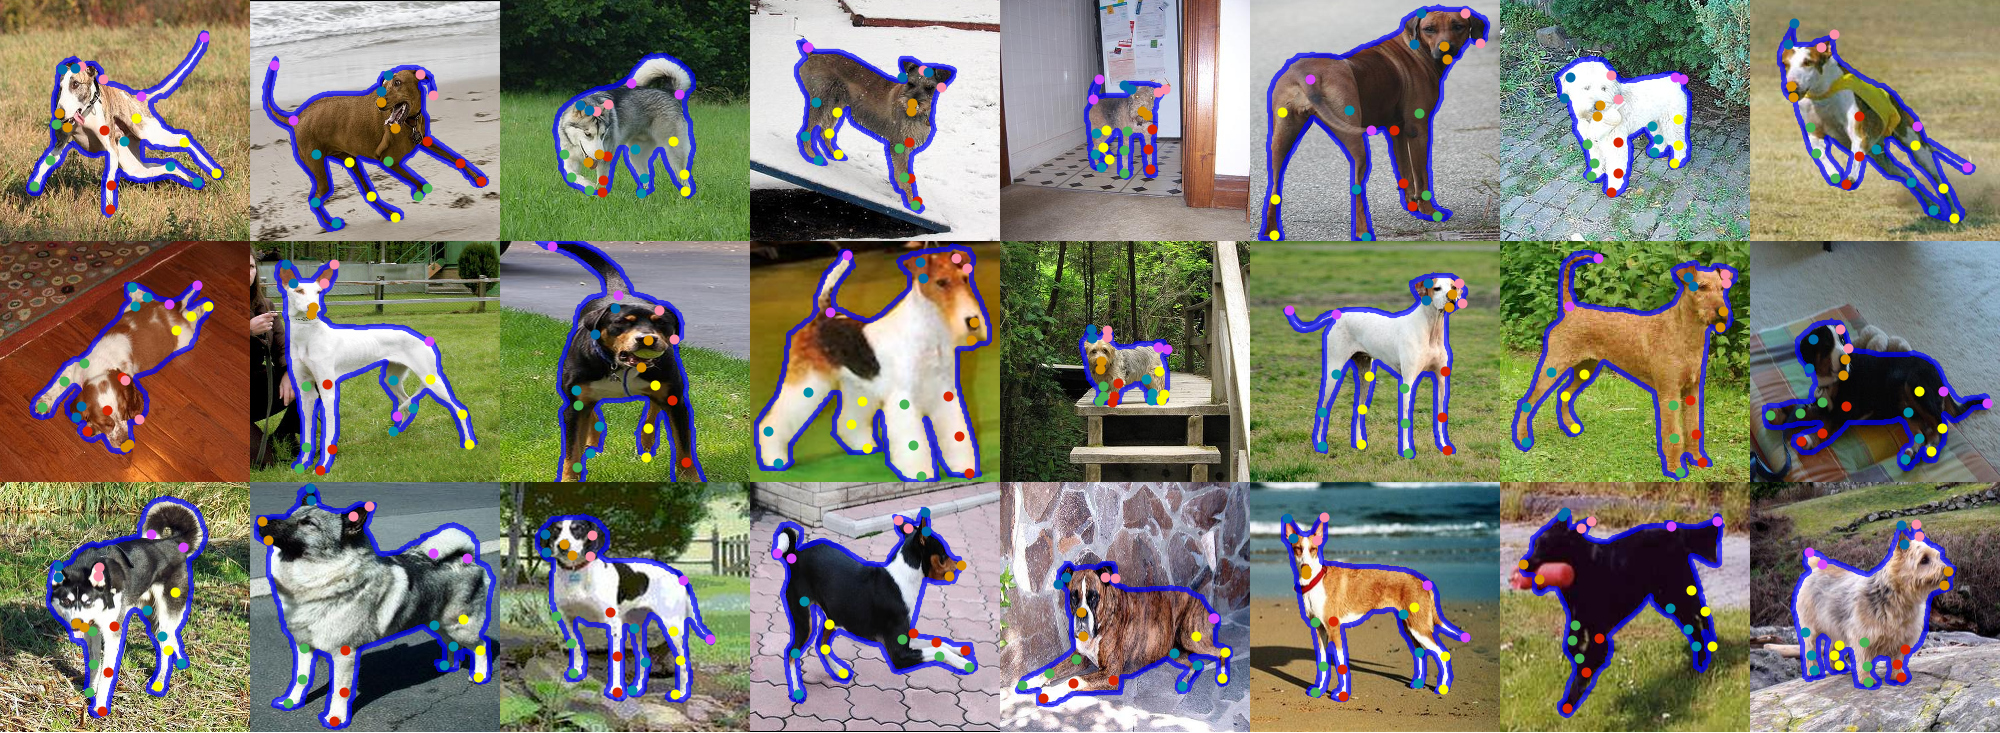
\includegraphics[height=0.1775\textheight]{figures/collage_wide.jpg}
      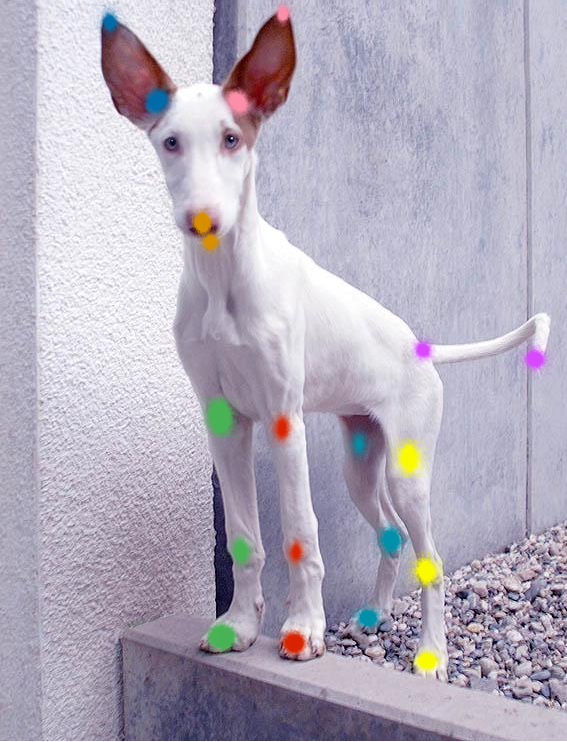
\includegraphics[height=0.1775\textheight]{figures/heatmap.png}
      \caption{\textbf{StanfordExtra example images}. \emph{Left}: outlined segmentations and labelled keypoints for a selection of StanfordExtra images. \emph{Right}: heatmap showing annotator uncertainty in per-keypoint clicking, computed over the entire dataset.}
      \label{fig:dataset}
  \end{figure*}
  
  In order to evaluate our method, we introduce StanfordExtra: a new large-scale dataset with annotated 2D keypoints and binary segmentation masks for dogs. We opted to take source images from the existing Stanford Dog Dataset~\cite{StanfordDogs}, which consists of 20,580 dog images taken `in the wild' and covers 120 dog breeds. The dataset contains vast shape and pose variation between dogs, as well as nuisance factors such as self/environmental occlusion, interaction with humans/other animals and partial views. Figure~\ref{fig:dataset} (left) shows samples from the new dataset.
  
  We used Amazon Mechanical Turk to collect a binary silhouette mask and 20 keypoints per image: 3 per leg (knee, ankle, toe), 2 per ear (base, tip), 2 per tail (base, tip), 2 per face (nose and jaw). We can approximate the difficulty of the dataset by analysing the variance between 3 annotators at both the joint labelling and silhouette task. Figure~\ref{fig:dataset} (right) illustrates typical per-joint variance in joint labelling. Further details of the data curation procedure are left to the supplementary materials. 
  
  \subsection{Evaluation protocol}
  
  Our evaluation is based on our new StanfordExtra dataset. In line with other methods which tackle `in the wild' 3D reconstruction of articulated subjects~\cite{kolotouros2019learning,kolotouros19convolutional}, we filter images from the original dataset of 20,580 for which the majority of dog keypoints are invisible. We consider these images unsuitable for our full-body dog reconstruction task. We also remove images for which the consistency in keypoint/silhouette segmentations between the 3 annotators is below a set threshold. This leaves us with 8,476 images which we divide per-breed into an 80\%/20\% train and test split.
  
  We consider two primary evaluation metrics. IoU is the intersection-over-union of the projected model silhouette compared to the ground truth annotation and indicates the quality of the reconstructed 3D shape. Percentage of Correct Keypoints (PCK) computes the percentage of joints which are within a normalized distance (based on square root of 2D silhouette area) to the ground truth locations, and evaluates the quality of reconstructed 3D pose. We also produce PCK results on various joint groups (legs, tail, ears, face) to compare the reconstruction accuracy for different parts of the dog model.
  
  \subsection{Training procedure}
  
  We train our model in two stages. The first omits the silhouette loss which we find can lead the network to unsatisfactory local minima if applied too early. With the silhouette loss turned off, we find it satisfactory to use the simple unimodal prior (and without EM) for this preliminary stage since there is no loss to specifically encourage a strong shape alignment. After this, we introduce the silhouette loss, the mixture prior and begin applying the expectation maximization updates over $M=10$ clusters. We train the first stage for 250 epochs, the second stage for 150 and apply the EM step every 50 epochs. All losses are weighted, as described in the supplementary. The entire training procedure takes 96 hours on a single P100 GPU.
  
  
  
  \subsection{Comparison to baselines}
  
  We first compare our method to various baseline methods. SMAL~\cite{DBLP:journals/corr/ZuffiKJB16} is an approach which fits the 3D SMAL model using per-image energy minimization. Creatures Great and SMAL (CGAS)~\cite{biggs2018creatures} is a three-stage method, which employs a joint predictor on silhouette renderings from synthetic 3D dogs, applies a genetic algorithm to clean predictions, and finally applies the SMAL optimizer to produce the 3D mesh.
  
  At test-time both SMAL and CGAS rely on manually-provided segementation masks, and SMAL also relies on hand-clicked keypoints. In order to produce a fair comparison, we produce a set of \emph{predicted} keypoints for StanfordExtra by training the Stacked Hourglass Network~\cite{newell2016stacked} with 8 stacks and 1 block, and \emph{predicted} segmentation masks using DeepLab v3+~\cite{journals/corr/ChenPK0Y16}. The Stacked Hourglass Network achieves 71.4\% PCK score, DeepLab v3+ achieves 83.4\% IoU score and the CGAS joint predictor achieves 41.8\% PCK score. 
  
  Table~\ref{tab:baselines} and Figure~\ref{fig:comparison_sup} show the comparison against competitive methods. For full examination, we additionally provide results for SMAL and CGAS in the scenario that ground-truth keypoints and/or segmentations are available at test time. 
  The results show our end-to-end method outperforms the competitors when they are provided with predicted keypoints/segmentations (white rows). Our method therefore achieves a new state-of-the-art on this 3D reconstruction task. In addition, we show our method achieves improved average IoU/PCK scores than competitive methods, even when they are provided ground truth annotations at test time (grey rows). We also demonstrate wider applicability of two contributions from our work (scale parameters and improved prior) by showing improved performance of the SMAL method when these are incorporated. Finally, our model's test-time speed is significantly faster than the competitors as it does not require an optimizer.
  
  \begin{table}[]
{
    \small
    \centering
    \begin{tabular}{@{}lcccccccc@{}}
    \toprule
    \multicolumn{1}{l}{Method} & 
    \multicolumn{1}{c}{Kps} & 
    \multicolumn{1}{c}{Seg} & 
    \multicolumn{1}{c}{IoU} & 
    \multicolumn{5}{c}{PCK} \\
    \multicolumn{4}{c}{} &
    \multicolumn{1}{c}{Avg} &
    \multicolumn{1}{c}{Legs} &
    \multicolumn{1}{c}{Tail} &
    \multicolumn{1}{c}{Ears} &
    \multicolumn{1}{c}{Face} \\
    \midrule
    SMAL~\cite{zuffi2017menagerie} & Pred & Pred & 67.9 & 67.1 & 65.7 & 79.5 & 54.9 & 87.4  \\
    SMAL & GT & GT &  69.2 & 72.6 & 69.9 & \textbf{92.0} & 58.6 & \textbf{96.9} \\
    SMAL & GT & Pred & 68.6 & 72.6 & 70.2 & 91.5 & 58.1 & \textbf{96.9} \\ 
    SMAL & Pred & GT & 68.5 & 67.4 & 66.0 & 79.9 & 55.0 & 88.2 \\ 
    % \rowcolor[gray]{.9} SMAL & GT & GT &  69.2 & 72.6 & 69.9 & \textbf{92.0} & 58.6 & \textbf{96.9} \\
    % \rowcolor[gray]{.9} SMAL & GT & Pred & 68.6 & 72.6 & 70.2 & 91.5 & 58.1 & \textbf{96.9} \\ 
    % \rowcolor[gray]{.9} SMAL & Pred & GT & 68.5 & 67.4 & 66.0 & 79.9 & 55.0 & 88.2 \\ 
    \hline
    CGAS~\cite{biggs2018creatures} & CGAS & Pred & 62.4 & 43.7 & 46.5 & 64.1 & 36.5 & 21.4  \\
    % \rowcolor[gray]{.9} CGAS & CGAS & GT & 63.1 & 43.6 & 46.3 & 64.2 & 36.3 & 21.6 \\
    CGAS & CGAS & GT & 63.1 & 43.6 & 46.3 & 64.2 & 36.3 & 21.6 \\
    \hline
    % \rowcolor[gray]{.9} SMAL + scaling & Pred & Pred & 69.3 & 69.6 & 69.4 & 79.3 & 56.5 & 87.6 \\
    % \rowcolor[gray]{.9} SMAL + scaling + new prior & Pred & Pred & 70.7 & 71.6 & 71.5 & 80.7 & 59.3 & 88.0 \\
    SMAL + scaling & Pred & Pred & 69.3 & 69.6 & 69.4 & 79.3 & 56.5 & 87.6 \\
    SMAL + scaling + new prior & Pred & Pred & 70.7 & 71.6 & 71.5 & 80.7 & 59.3 & 88.0 \\
    \hline
    \textbf{Ours} & --- & --- & \textbf{73.6} & \textbf{75.7} & \textbf{75.0} & 77.6 & \textbf{69.9} & 90.0 \\
    \bottomrule 
    \end{tabular}
    \vspace{1em}
    \caption{\label{tab:baselines}\textbf{Baseline comparisons.} Both PCK and silhouette IOU scores are shown for SOTA methods under varying conditions. A combination of both ground truth (GT) and predicted (Pred) keypoints/segmentations using hourglass network and deeplab respectively. For the CGAS method we also test using their keypoint predictor (CGAS). The addition of scaling and new prior are shown to improve the original SMAL method.}
}
\end{table}
  \input{fig_comparison_sup_cr}
  
  
  
  \subsection{Generalization to unseen dataset}
  
  Table~\ref{tab:animalpose} shows an experiment to compare how well our model generalizes to a new data domain. We test our model against the SMAL~\cite{DBLP:journals/corr/ZuffiKJB16} method (using predicted keypoints and segmentations as above for fairness) on the recent Animal Pose dataset~\cite{animalpose}. The data preparation process is the same as for StanfordExtra and no fine-tuning was used for either method. We achieve strong results in this unseen domain and still improve over the SMAL optimizer.
  
  \begin{table}[t!]
      \parbox{.45\linewidth}{
          \centering
          \begin{tabular}{@{}lcccccc@{}}
          \toprule
          \multicolumn{1}{l}{Method} & 
          \multicolumn{1}{c}{IoU} & 
          \multicolumn{5}{c}{PCK} \\
          \multicolumn{2}{c}{} &
          \multicolumn{1}{c}{Avg} &
          \multicolumn{1}{c}{Legs} &
          \multicolumn{1}{c}{Tail} &
          \multicolumn{1}{c}{Ears} &
          \multicolumn{1}{c}{Face} \\
          \midrule
          SMAL~\cite{DBLP:journals/corr/ZuffiKJB16} & 63.6 & 69.1 & 60.9 & 83.5 & 75.0 & 93.0 \\
          % \hline
          \textbf{Ours} & \textbf{66.9} & \textbf{73.8} & \textbf{65.1} & \textbf{85.6} & \textbf{84.0} & \textbf{93.6} \\
          \bottomrule
          \multicolumn{7}{c}{} \\
          \multicolumn{7}{c}{}
          \end{tabular}
          \vspace{1em}
          \caption{
              \label{tab:animalpose}
              \textbf{Animal Pose dataset~\cite{animalpose}}. Evaluation on recent Animal Pose dataset with no fine-tuning to our method nor joint/silhouette predictors used for SMAL.}
      }
      \hfill
      \parbox{.45\linewidth}{
          % \small
          \centering
          \begin{tabular}{@{}lcccccc@{}}
          \toprule
          \multicolumn{1}{l}{Method} & 
          \multicolumn{1}{c}{IoU} & 
          \multicolumn{5}{c}{PCK} \\
          \multicolumn{2}{c}{} &
          \multicolumn{1}{c}{Avg} &
          \multicolumn{1}{c}{Legs} &
          \multicolumn{1}{c}{Tail} &
          \multicolumn{1}{c}{Ears} &
          \multicolumn{1}{c}{Face} \\
          \midrule
          \textbf{Ours} & \textbf{73.6} & \textbf{75.7} & \textbf{75.0} & \textbf{77.6} & 69.9 & 90.0 \\
          $-$EM & 67.7 & 74.6 & 72.9 & 75.2 & \textbf{72.5} & 88.3 \\
          $-$MoG & 68.0 & 74.9 & 74.3 & 73.3 & 70.0 & \textbf{90.2} \\ 
          $-$Scale & 67.3 & 72.6 & 72.9 & 75.3 & 62.3 & 89.1 \\
          \bottomrule 
          \end{tabular}
          \vspace{1em}
          \caption{\label{tab:ablation}\textbf{Ablation study.} Evaluation with the following contributions removed: (a) EM updates, (b) Mixture Shape Prior, (c) SMBLD scale parameters.}
      }
  \end{table}
  
  
  
  \subsection{Ablation study}
  
  We also produce a study in which we ablate individual components of our method and examine the effect on the PCK/IoU performance. We evaluate three variants: (1) \textbf{Ours w/o EM} that omits EM updates, (2) \textbf{Ours w/o MoG} which replaces our mixture shape prior with a unimodal prior, (3)~\textbf{Ours w/o Scale} which removes the scale parameters. 
  
  The results in Table~\ref{tab:ablation} indicate that each individual component has a positive impact on the overall method performance. In particular, it can be seen that the inclusion of the EM and mixture of Gaussians prior leads to an improvement in IoU, suggesting that the shape prior refinements steps help the model accurately fit the exact dog shape. Interestingly, we notice that adding the mixture of Gaussians prior but omitting EM steps slightly hinders performance, perhaps due to a sub-optimal initialization for the $M$ clusters. However, we find adding EM updates to the mixture of Gaussian model improves all metrics except the ear keypoint accuracy. We observe the error here is caused by the our shape prior learning slightly imprecise shapes for dogs with extremely `floppy' ears. Although there is good silhouette coverage for these regions, the fact our model has only a single articulation point per ear causes a lack of flexibility that results in occasionally misplaced ear tips for these instances. This could be improved in future work by adding additional model joints to the ear. Finally, our results show the increased model flexibility afforded by the SMBLD scale parameters has a positive effect on IoU/PCK scores. 
  
  
  \subsection{Qualitative evaluation}
  
  Figure~\ref{fig:comparison_sup} shows a range of predicted 3D reconstructions from our method when tested on a wide range of StanfordExtra and Animal Pose~\cite{animalpose} dogs. The examples include challenging poses, large diversity in dog shape and size, interaction with humans, various environmental conditions and handling occluded keypoints. Note that only StanfordExtra is used for training and we use no fine-tuning to produce results on the Animal Pose dataset.
  
  \section{Conclusions}
  This paper presents an end-to-end method for automatic, monocular 3D dog reconstruction. We achieve this using only weak 2D supervision, provided by our novel StanfordExtra dataset. Furthermore, we show we can learn a more detailed shape prior by tuning a Gaussian mixture during model training and this leads to improved reconstructions. We also show our method improves over competitive baselines, even when they are given access to ground truth data at test time.
  
  Future work should involve tackling some failure cases of our system, for example handling multiple overlapping dogs or dealing with heavy motion blur. Other areas for research include extending our EM formulation to handle video input to take advantage of multi-view shape constraints, and transferring knowledge accumulated through training on StanfordExtra dogs to other species.